\section{Ensuring the method is robust}
\label{sec:robustness}

The above results are quite striking; only around 50\% of the gaseous
mass in a given halo (at Milky-Way halo mass). To ensure that the methodology
discussed above is robust, several extra checks have been put in place, that
are discussed below.

\subsection{Expanding the halo boundary}

A possible criticism of the above definition of lagrangian regions is that
they are too sensitive to halo boundary effects. In the above analysis, dark
matter particles are identified as belonging to the lagrangian region of a
given halo if they lie within the virial radius of that halo at $z=0$. In
this section, changing the radius at which particles are selected to be part
of the eventual lagrangian region is explored.

\begin{figure}
    \centering
    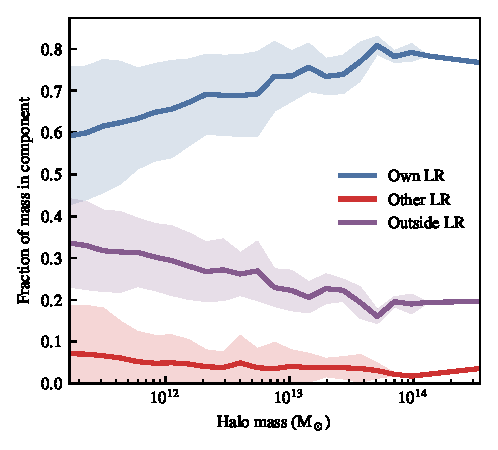
\includegraphics[width=\columnwidth]{generated_figures/12_rvir_only_lr/component_fraction_vs_halo_mass_both.pdf}
    \caption{The analogue of Figure \ref{fig:massfrac} but after re-running
    the analysis with lagrangian regions re-defined such that $r_{\rm vir,
    new} = 1.2 r_{\rm vir, old}$, see the text for details. The dashed lines
    represent the exact curves as shown in Figure \ref{fig:massfrac} for
    direct comparison by the reader. Similar trends follow if the lagrangian
    region is extended to include particles that lie within 1.5\rvir{}.}
    \label{fig:comparevirialradii}
\end{figure}

The procedure for extending the lagrangian region is as follows:
\begin{enumerate}
    \item For every halo in the box, search for the centre of that halo (by
          looking for the extreme particles in each direction and finding
          their centre point, as well as taking into account the periodic
          boundaries), and the corresponding radius. This is used instead of the
          halo centers from AHF to ensure the code remains generic, and provides
          the same data.
    \item Multiply this radius (which by definition, from the halo finder, is
          the virial radius \rvir{}) by a factor, such as 1.2, or 1.5
    \item For each halo in the box, use a periodic KDTree to search for the
          neighbours of the centre point within that radius, going from
          highest mass (in dark matter) to lowest mass to ensure that
          lower-mass halos `steal' from the higher mass ones, should they
          be embedded or nearby. From this we would expect to see slightly
          increased transfer from other regions.
    \item Label these particles as belonging to the lagrangian region of
          that halo, but not to the halo themselves if they lie outside
          of \rvir{}.
    \item Re-run the original analysis with this definition of the particles that
          that lagrangian region.
\end{enumerate}

In Figure \ref{fig:comparevirialradii}, the baryonic mass fraction from each
lagrangian component is shown as a function of halo mass, where the
lagrangian region has been extended to include particles within 1.2\rvir{} of
the halo centre. Note that no extra particles are included in the halo, i.e.
the halo definition still ends at \rvir{}. This ensures that the same edge
effects that we are trying to remove are not simply present at the increased
radius. This also means that the mass of the particles in the lagrangian
region is no longer the same as the mass of the particles in the final,
$z=0$, halo; there will necessarily be a higher fraction of mass originating
from the lagrangian region that is defined by the larger volume.

Figure \ref{fig:comparevirialradii} shows that around 5\% of the mass of the
halo has been re-characterised as originating in the same lagrangian region
as the one that the halo defines instead of originating outside any lagrangian
region. There has been little change in the mass originating from the
lagrangian regions defined by other halos, which shows that there has been
very little `stealing' of material when the re-definition of the lagrangian
region took place.

The same overall trends with halo mass are observed even with this extended
definition for the lagrangian region, with the expected change observed; there
will be some gas in the CGM that is strongly mixed on the halo boundary.

\subsection{The definition of lagrangian region}

\begin{figure}
    \centering
    \includegraphics[width=\columnwidth]{generated_figures/neighbour_search/neighbour_search/component_fraction_vs_halo_mass_comparison.pdf}
    \caption{The analogue of Figure \ref{fig:massfrac}, but with lagrangian
    regions filled out with a local nearest neighbour search of the nearest
    $n=$1 (i.e. only the particle itself), 2, 4, 8, 16, 32, and 64 particles,
    with the lines getting lighter as more particles are included in the
    smoothing. Note the general trend of the mass fraction from the
    lagrangian region of a halo increasing as they are filled out by the
    smoothing, with the fraction from other lagrangian regions remaining
    relatively unchanged.}
    \label{fig:filledlrmass}
\end{figure}

In the above analysis, we considered a very diffuse notion of a lagrangian
region, defined particle-by-particle. The definition of what constitutes a
lagrangian region is somewhat open to interpretation; there may be particles
enclosed in the convex hull of such a region that do not end up in the
collapsed object, especially if an incorrect choice is made for the
gravitational softening. Whilst increasing the virial radius will go some way
to filling the `holes' in these regions, due to the large transfer of dark
matter that still occurs (\S \ref{sec:haloindependent}), a different
methodology is required.

Some of the holes that are present in lagrangian regions are vitally important;
these holes will collapse down to independent halos. An effort must be made to
ensure that those holes remain, whilst others are erased, with lower-mass halos
taking priority over their higher-mass cousins. With this hole-filling
exercise, it is important to note that even dark matter particles may now have
a different halo ID to lagrangian ID. The methodology that is proposed here is
as follows:
\begin{enumerate}
    \item Initially define lagrangian regions in the same way as before for
          the dark matter.
    \item Find the first $n$ neighbours of every dark matter particle which
          has a lagrangian region ID of -1, i.e. it is outside of any region.
    \item Overwrite the lagrangian ID of these particles with the lowest (i.e.
          corresponding to the lowest mass halo) in the group.
    \item Extend the lagrangian region definition to the gas particles in
          the same way as previously, by finding the closest gas neighbour
	  particle to every dark matter particle.
\end{enumerate}
This aims to both fill out the lagrangian regions, increasing their
volume-filling fraction, ensure that no particles are `stolen' from higher-mass
halos, and reduce surface effects leading to spurious lagrangian transfer from
outside any region. See Figure \ref{fig:filledlrmass} for the results for
$n=1$ to $n=64$ neighbours.

The effect of this smoothing, by design, is to move more particles from outside
any lagrangian region to within one. Hence, we see significant movement of
mass being labelled as originating outside any lagrangian region to originating
inside the lagrangian region of the host halo. This is expected as the surface
of the lagrangian regions grow in the initial conditions, as well as particles that
lie within the convex hull of the initial lagrangian region being considered as
part of that region.

The more surprising result from this is that the fraction of baryonic mass in a
halo originating from another lagrangian region is almost constant throughout
this process. This implies, as we fill the regions from low-mass to high-mass,
that this transfer is extremely robust; we would expect to see huge gains if
it was that halos with only a few particles were being extended to include many
more particles than they should.
